\documentclass[10pt,aspectratio=169]{beamer}

\usetheme{Boadilla}
\usecolortheme{default}
\usefonttheme{professionalfonts}
\usepackage[T1]{fontenc}
\usepackage{lmodern}
\usepackage{amsmath,amssymb,bm}
\usepackage{booktabs}
\usepackage{tikz}
\usetikzlibrary{arrows.meta,positioning,calc,fit,shapes.geometric}
\usepackage{appendixnumberbeamer}

\definecolor{navy}{RGB}{22,45,78}
\definecolor{blue}{RGB}{54,119,184}
\definecolor{green}{RGB}{35,139,69}
\definecolor{orange}{RGB}{221,122,1}
\definecolor{red}{RGB}{201,60,60}
\definecolor{purple}{RGB}{115,63,165}
\setbeamercolor{structure}{fg=navy}
\setbeamercolor{frametitle}{fg=navy}
\setbeamercolor{title}{fg=navy}
\setbeamercolor{alerted text}{fg=red}
\setbeamertemplate{navigation symbols}{}
\setbeamertemplate{footline}{\hfill\color{gray}\insertshorttitle\quad|\quad\insertframenumber\,/\,\inserttotalframenumber\hspace{1.2em}\vspace{0.8em}}
\setbeamertemplate{itemize items}[circle]
\setlength{\leftmargini}{1.2em}
\graphicspath{{artifacts/mh01_graphs/}{../artifacts/mh01_graphs/}}

\newcommand{\fig}[2]{\begin{center}\includegraphics[width=#1\linewidth,height=.64\textheight,keepaspectratio]{#2}\end{center}}
\newcommand{\smallcite}[1]{\vfill\hfill\scriptsize\color{gray}#1}
\newcommand{\secheader}[1]{\begin{center}\color{navy}\Large\textbf{#1}\end{center}}

\title[Visual-Inertial ESEKF SLAM]{Visual-Inertial ESEKF SLAM\\from First Principles}
\subtitle{A verified stereo-inertial pipeline, its real-data behavior, and an honest consistency diagnosis}
\author{Imad Dar}
\institute{Technical deep dive}
\date{\today}

\begin{document}

\begin{frame}
  \titlepage
\end{frame}

\begin{frame}{The question: can a small estimator be trustworthy enough to teach from?}
  \begin{columns}[T]
    \column{0.55\textwidth}
    \Large Build a visual-inertial SLAM system from scratch, then make every important claim testable.
    \vspace{0.7em}
    \normalsize
    \begin{itemize}
      \item Stereo camera: geometric constraints, but intermittent and data-association dependent.
      \item IMU: high-rate motion prediction, but bias turns into rapid position drift.
      \item Target: an offline EuRoC pipeline that can become a real-time ROS 2 system.
    \end{itemize}
    \column{0.42\textwidth}
    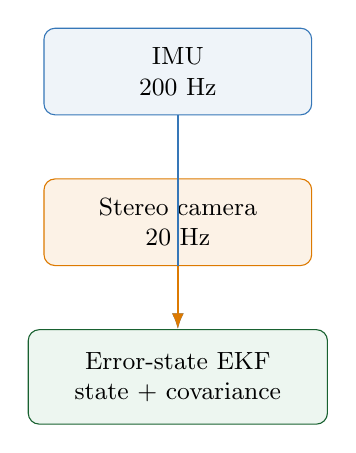
\begin{tikzpicture}[node distance=8mm, every node/.style={align=center,font=\small}]
      \node[draw=blue, rounded corners, fill=blue!8, minimum width=34mm, minimum height=11mm] (imu) {IMU\\200 Hz};
      \node[draw=orange, rounded corners, fill=orange!10, minimum width=34mm, minimum height=11mm, below=of imu] (cam) {Stereo camera\\20 Hz};
      \node[draw=green!70!black, rounded corners, fill=green!8, minimum width=38mm, minimum height=12mm, below=of cam] (ekf) {Error-state EKF\\state + covariance};
      \draw[-{Latex[length=2mm]}, thick, blue] (imu) -- (ekf);
      \draw[-{Latex[length=2mm]}, thick, orange] (cam) -- (ekf);
    \end{tikzpicture}
  \end{columns}
\end{frame}

\begin{frame}{The hard part is not integrating motion; it is managing uncertainty}
  \begin{columns}[T]
    \column{0.54\textwidth}
    \begin{itemize}
      \item Accelerometer bias is integrated twice into position.
      \item Gyroscope bias rotates gravity into a false horizontal acceleration.
      \item Vision can correct drift only if projection, frames, Jacobians, and covariance all agree.
    \end{itemize}
    \vspace{0.5em}
    \alert{A plausible trajectory is not evidence that the covariance is correct.}
    \column{0.44\textwidth}
    \begin{block}{Design goal}
      Every layer gets an independent test oracle: analytic truth, finite differences, dense batch update, or Monte Carlo.
    \end{block}
  \end{columns}
\end{frame}

\begin{frame}{The project is an end-to-end visual-inertial system}
  \centering
  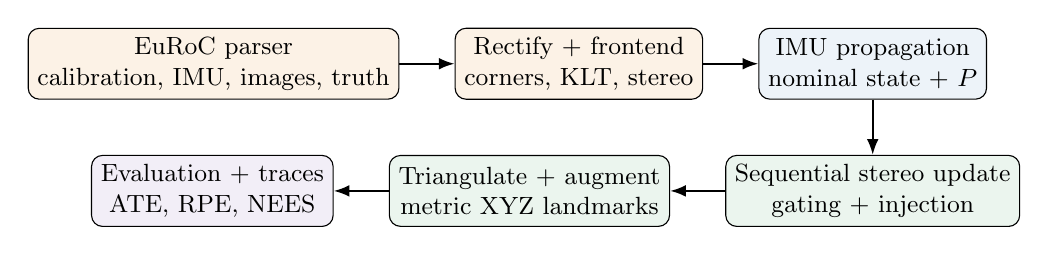
\begin{tikzpicture}[node distance=7mm, every node/.style={draw, rounded corners, minimum height=9mm, align=center, font=\small}]
    \node[fill=orange!10] (parse) {EuRoC parser\\calibration, IMU, images, truth};
    \node[fill=orange!10, right=of parse] (front) {Rectify + frontend\\corners, KLT, stereo};
    \node[fill=blue!9, right=of front] (prop) {IMU propagation\\nominal state + $P$};
    \node[fill=green!9, below=of prop] (update) {Sequential stereo update\\gating + injection};
    \node[fill=green!9, left=of update] (augment) {Triangulate + augment\\metric XYZ landmarks};
    \node[fill=purple!9, left=of augment] (eval) {Evaluation + traces\\ATE, RPE, NEES};
    \draw[-{Latex[length=2mm]}, thick] (parse) -- (front);
    \draw[-{Latex[length=2mm]}, thick] (front) -- (prop);
    \draw[-{Latex[length=2mm]}, thick] (prop) -- (update);
    \draw[-{Latex[length=2mm]}, thick] (update) -- (augment);
    \draw[-{Latex[length=2mm]}, thick] (augment) -- (eval);
  \end{tikzpicture}
  \vspace{1em}
  \begin{itemize}
    \item Implemented: parser, rectification, KLT frontend, propagation, stereo update, augmentation, full MH\_01 evaluator.
    \item Not implemented: marginalization, FEJ/OC-EKF, iterated EKF, ROS 2 deployment.
  \end{itemize}
\end{frame}

\section{Estimator formulation}

\begin{frame}{The nominal state lives on $SO(3)$; the filter estimates a local error}
  \begin{columns}[T]
    \column{0.50\textwidth}
    \[
      x = \left[p_W, v_W, R_{WB}, b_a, b_g\right]
    \]
    \[
      \delta x = \left[\delta p_W, \delta v_W, \delta\theta_B, \delta b_a, \delta b_g\right] \in \mathbb{R}^{15}
    \]
    \begin{itemize}
      \item Position, velocity, and biases are additive.
      \item Rotation is corrected multiplicatively:
      \[R_{WB} \leftarrow R_{WB}\exp(\delta\theta_B^\wedge).\]
    \end{itemize}
    \column{0.47\textwidth}
    \begin{block}{Why error-state?}
      A 3D local rotation error has an ordinary Gaussian covariance; the nominal rotation remains a valid element of $SO(3)$ after every update.
    \end{block}
    \begin{alertblock}{Convention is load-bearing}
      $\delta\theta$ is body-frame, right-multiplied. Mixing left and right perturbations can pass trivial tests and still corrupt a real filter.
    \end{alertblock}
  \end{columns}
\end{frame}

\begin{frame}{Propagation uses IMU measurements to advance state and covariance}
  \begin{columns}[T]
    \column{0.56\textwidth}
    \[
      a_W = R_{WB}(a_m-b_a-n_a)+g_W
    \]
    \[
      p^+ = p + v\Delta t + \tfrac12a_W\Delta t^2,\quad v^+=v+a_W\Delta t
    \]
    \[
      R^+=R\exp((\omega_m-b_g-n_g)\Delta t)^\wedge
    \]
    \[
      P^+ = \Phi P\Phi^T + Q_d,\quad \Phi\approx I+F\Delta t
    \]
    \column{0.40\textwidth}
    \begin{itemize}
      \item Nominal state is integrated on the manifold.
      \item Covariance is propagated in the 15D local error coordinates.
      \item First-order $\Phi$ is a deliberate, measured trade-off.
    \end{itemize}
  \end{columns}
\end{frame}

\begin{frame}{Stereo converts matched pixels into a metric geometric constraint}
  \begin{columns}[T]
    \column{0.50\textwidth}
    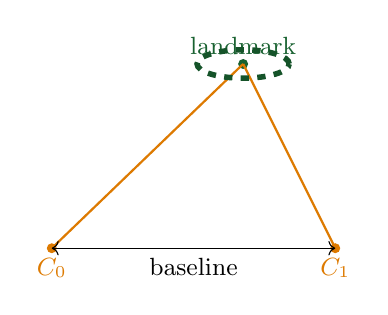
\begin{tikzpicture}[scale=0.9, every node/.style={font=\small}]
      \coordinate (c0) at (0,0); \coordinate (c1) at (4,0); \coordinate (l) at (2.7,2.6);
      \fill[orange] (c0) circle (2pt) node[below] {$C_0$};
      \fill[orange] (c1) circle (2pt) node[below] {$C_1$};
      \fill[green!70!black] (l) circle (2pt) node[above] {landmark};
      \draw[orange, thick] (c0)--(l); \draw[orange, thick] (c1)--(l);
      \draw[<->] (c0)--node[below] {baseline} (c1);
      \draw[green!60!black, dashed, line width=2pt] (l) ellipse (0.65 and 0.20);
    \end{tikzpicture}
    \column{0.46\textwidth}
    \begin{itemize}
      \item Rectification makes correspondence a row-constrained search.
      \item Disparity gives metric depth, but depth uncertainty grows along the viewing ray.
      \item New landmarks inherit uncertainty from pixels \emph{and} robot pose.
    \end{itemize}
  \end{columns}
\end{frame}

\begin{frame}{A camera update is a pixel-space correction}
  \begin{columns}[T]
    \column{0.53\textwidth}
    For a landmark $p_L^W$, project it into both rectified cameras:
    \[
      y = \begin{bmatrix}u_0&v_0&u_1&v_1\end{bmatrix}^T,
      \quad \nu = y-h(\hat{x})
    \]
    \[
      S=HPH^T+R,\quad K=PH^TS^{-1}
    \]
    \[
      \delta x = K\nu,\quad P\leftarrow(I-KH)P(I-KH)^T+KRK^T
    \]
    \column{0.43\textwidth}
    \begin{block}{Interpretation}
      The innovation asks: ``How surprising is this pixel observation under the current state and covariance?''
    \end{block}
    \begin{alertblock}{Gate}
      Reject an observation when $\nu^TS^{-1}\nu$ exceeds the 4-dof chi-square threshold.
    \end{alertblock}
  \end{columns}
\end{frame}

\begin{frame}{Sequential updates preserve a useful batch-update oracle}
  \begin{itemize}
    \item A frame can contain many landmarks, but each stereo observation has only nine non-zero state columns.
    \item The implementation freezes the nominal linearization point at frame entry, sweeps landmarks sequentially, and injects one accumulated error at the end.
    \item That design makes the sequential result equal the dense batch update for the same frame; a test verifies agreement to $10^{-12}$.
  \end{itemize}
  \vspace{1em}
  \begin{block}{Why this matters in an interview}
    The batch path is not production code. It is a high-cost oracle that narrows an inconsistency from ``somewhere in the filter'' to a specific component.
  \end{block}
\end{frame}

\section{How the system is verified}

\begin{frame}{The test strategy targets failure modes, not just coverage}
  \begin{tabular}{p{0.31\linewidth}p{0.56\linewidth}}
    \toprule
    Evidence & What it can falsify \\
    \midrule
    Analytic synthetic truth & Integrator order, gravity sign, bias removal \\
    Central differences & Frame/sign/order mistakes in projection Jacobians \\
    Dense batch oracle & Sequential sweep or accumulated-error mistakes \\
    Monte Carlo covariance & Transposed, sign-flipped, or mis-scaled $F/Q$ blocks \\
    EuRoC MH\_01 & Parser, calibration, frontend, timing, and closed-loop behavior \\
    \bottomrule
  \end{tabular}
  \vspace{1em}
  \begin{alertblock}{Verification principle}
    The strongest tests compare independently produced behavior, not two versions of the same algebra.
  \end{alertblock}
\end{frame}

\begin{frame}{Monte Carlo makes covariance claims falsifiable}
  \fig{0.73}{08_covariance_monte_carlo_margin.png}
  \smallcite{Correct propagation: three seeded runs. Corrupted-$F$ bar: minimum observed deviation over single-block corruptions.}
\end{frame}

\begin{frame}{The measured integrator order matches the chosen discretization}
  \fig{0.62}{09_integrator_convergence.png}
  \begin{itemize}
    \item Halving $\Delta t$ halves the combined position/velocity error.
    \item The second-order position term improves the constant, not the global order of the method.
  \end{itemize}
\end{frame}

\section{Real-data results}

\begin{frame}{MH\_01 runs end-to-end in the raw EuRoC world frame}
  \fig{0.80}{01_trajectory_overlay.png}
  \smallcite{Truth-initialized full MH\_01 run. No global SE(3) alignment: alignment would hide drift.}
\end{frame}

\begin{frame}{A Kalman update has a prior, a posterior, and uncertainty geometry}
  \fig{0.78}{02_kalman_update_in_action.png}
  \smallcite{The figure shows state-space prior/posterior and 2-sigma position covariance. The actual camera observation remains in pixel space.}
\end{frame}

\begin{frame}{The real run exposes over-confidence rather than hiding it}
  \fig{0.84}{03_error_and_uncertainty.png}
  \begin{itemize}
    \item After roughly 50 seconds, position error is much larger than reported 1-sigma position uncertainty.
    \item This is an observation from one real trajectory; the controlled Monte Carlo experiment supports the statistical consistency claim.
  \end{itemize}
\end{frame}

\begin{frame}{Camera updates are visible as small, frequent posterior corrections}
  \fig{0.81}{05_camera_update_effect.png}
  \smallcite{Prior is the IMU-propagated camera-time state; posterior is after the visual sweep.}
\end{frame}

\begin{frame}{Gating reveals the estimator's view of innovation consistency}
  \fig{0.80}{06_innovation_gating.png}
  \begin{itemize}
    \item Applied observations lie predominantly below the 4-dof chi-square gate.
    \item Gating is a covariance-aware consistency check, not a replacement for frontend outlier rejection.
  \end{itemize}
\end{frame}

\begin{frame}{Pixel innovations make the measurement model concrete}
  \fig{0.68}{07_pixel_innovations.png}
  \smallcite{Each gray segment is a predicted-to-observed left-camera pixel innovation for one accepted feature at one camera time.}
\end{frame}

\begin{frame}{Frontend health connects visual tracking to estimator updates}
  \fig{0.79}{13_frontend_health.png}
  \begin{itemize}
    \item Track count is not accuracy, but sudden loss constrains how much visual information the filter can receive.
    \item The acceptance fraction contextualizes the update count with the gate's decision.
  \end{itemize}
\end{frame}

\begin{frame}{The full trace separates position, velocity, attitude, and bias errors}
  \fig{0.79}{11_state_block_errors.png}
  \smallcite{Native units differ by block; compare within a panel, not across panels.}
\end{frame}

\begin{frame}{The covariance stays positive but becomes increasingly ill-conditioned}
  \fig{0.78}{14_covariance_numerical_health.png}
  \begin{itemize}
    \item Positive minimum eigenvalue is a necessary numerical-health condition.
    \item Conditioning is a monitoring signal; it is not itself proof of consistency.
  \end{itemize}
\end{frame}

\begin{frame}{NEES turns ``looks reasonable'' into a consistency question}
  \fig{0.80}{04_nees_over_time.png}
  \begin{block}{Read this correctly}
    A pointwise real-run NEES trace identifies over-confidence. A chi-square confidence interval applies to an ensemble mean, which is why the synthetic Monte Carlo control is essential.
  \end{block}
\end{frame}

\section{The negative result and diagnosis}

\begin{frame}{The closed-loop synthetic test improves drift but fails consistency}
  \begin{columns}[T]
    \column{0.48\textwidth}
    \begin{block}{Same 2-second scenario}
      \begin{itemize}
        \item Propagation-only final position error: \textbf{0.163 m}
        \item With camera updates: \textbf{0.0545 m}
        \item 195 applied observations; 5 gated
      \end{itemize}
    \end{block}
    \column{0.48\textwidth}
    \begin{alertblock}{But mean 15-dof NEES}
      \begin{center}
      \begin{tabular}{lcc}
        & Mean & 95\% interval \\
        Propagation only & 13.56 & [13.52, 16.56] \\
        With updates & \alert{24.23} & [13.52, 16.56] \\
      \end{tabular}
      \end{center}
    \end{alertblock}
  \end{columns}
\end{frame}

\begin{frame}{The failure is concentrated in attitude and bias, not position}
  \fig{0.85}{10_nees_summary_and_blocks.png}
  \smallcite{Synthetic 50-run Monte Carlo diagnostic. The left panel uses the 15-dof mean interval; the right uses expected 3 per 3-dof block.}
\end{frame}

\begin{frame}{Evidence rules out the most obvious explanations}
  \begin{enumerate}
    \item \textbf{Not propagation covariance:} the propagation-only control passes in the same harness.
    \item \textbf{Not sequential update mechanics:} sequential and dense batch agree to $10^{-12}$.
    \item \textbf{Not Jacobian convention algebra:} measurement Jacobians agree with central differences to $10^{-5}$.
    \item \textbf{Not gate selection bias:} widening the gate to infinity changes total NEES only $24.23\rightarrow23.66$.
    \item \textbf{Not yaw observability:} yaw NEES is 1.41 for expected 1.0; tilt NEES is 4.81 for expected 2.0.
  \end{enumerate}
\end{frame}

\begin{frame}{The diagnosis is first-order rotation linearization, not FEJ}
  \begin{columns}[T]
    \column{0.54\textwidth}
    \begin{itemize}
      \item Reducing initial tilt sigma from 0.01 rad to 0.001 rad moves total NEES from 24.23 to 15.92, inside the target interval.
      \item Tilt enters the camera model nonlinearly through rotation; position and landmark position are linear when $R$ is fixed.
      \item An iterated EKF relinearizes toward the posterior, targeting this measured second-order error.
    \end{itemize}
    \column{0.40\textwidth}
    \begin{block}{Engineering decision}
      Do not tune the consistency bound until it passes. Keep a regression ceiling and retain the statistical acceptance test as disabled future-work evidence.
    \end{block}
  \end{columns}
\end{frame}

\section{Takeaways}

\begin{frame}{What this project demonstrates}
  \begin{enumerate}
    \item \textbf{Estimator fluency:} manifold error states, stochastic IMU propagation, stereo projection, gated EKF updates, and landmark augmentation.
    \item \textbf{Systems fluency:} real image I/O, calibration/rectification, feature tracking, timing, data association, and reproducible traces.
    \item \textbf{Scientific discipline:} tests designed to fail under plausible mistakes, plus an explicit measurement of an unresolved limitation.
  \end{enumerate}
  \vspace{0.5em}
  \begin{alertblock}{Bottom line}
    A working trajectory is the start of estimator validation, not the end. The deliverable is a system whose errors are measurable, explainable, and actionable.
  \end{alertblock}
\end{frame}

\begin{frame}{The next iteration is targeted by evidence}
  \begin{columns}[T]
    \column{0.48\textwidth}
    \textbf{Estimator}
    \begin{itemize}
      \item Iterated EKF for tilt-linearization error.
      \item Static-start gravity alignment.
      \item Marginalization / bounded-map strategy.
    \end{itemize}
    \column{0.48\textwidth}
    \textbf{System}
    \begin{itemize}
      \item Calibrated frontend noise and stronger outlier rejection.
      \item Multi-sequence EuRoC evaluation.
      \item ROS 2 + Jetson timing validation.
    \end{itemize}
  \end{columns}
\end{frame}

\begin{frame}
  \centering
  \vfill
  {\color{navy}\Huge Thank you}
  \vspace{0.5em}

  \Large Questions
  \vfill
\end{frame}

\appendix
\section{Appendix}

\begin{frame}{Appendix: map of the deeper technical material}
  \begin{columns}[T]
    \column{0.48\textwidth}
    \begin{itemize}
      \item Frame and perturbation conventions
      \item Transition-matrix block structure
      \item Update sequence and reset Jacobian
      \item Stereo triangulation uncertainty
    \end{itemize}
    \column{0.48\textwidth}
    \begin{itemize}
      \item Full MH\_01 trace schema
      \item Metrics and their limitations
      \item Runtime/profile findings
      \item Interview questions and direct answers
    \end{itemize}
  \end{columns}
\end{frame}

\begin{frame}{Appendix: frame convention and perturbation rule}
  \begin{tabular}{ll}
    \toprule
    Quantity & Convention \\
    \midrule
    $p_W, v_W$ & Position and velocity expressed in world $W$ \\
    $R_{WB}$ & Rotates body-frame vectors into world frame \\
    $\delta\theta_B$ & Body-frame local orientation error \\
    $T_{BS}$ & Sensor-to-body rigid transform \\
    $P$ ordering & $[p,v,\theta,b_a,b_g]$ \\
    \bottomrule
  \end{tabular}
  \vspace{1em}
  \[
    R_{WB}^{\text{true}} = R_{WB}^{\text{estimate}}\exp(\delta\theta_B^\wedge)
  \]
  The finite-difference test intentionally rejects a left/global perturbation, preventing a convention mismatch from becoming a latent real-data bug.
\end{frame}

\begin{frame}{Appendix: the error transition matrix exposes the critical couplings}
  \scriptsize
  \[
  F = \begin{bmatrix}
  0&I&0&0&0\\
  0&0&-R[a-b_a]_\times&-R&0\\
  0&0&-[\omega-b_g]_\times&0&-I\\
  0&0&0&0&0\\
  0&0&0&0&0
  \end{bmatrix}
  \]
  \normalsize
  \begin{itemize}
    \item $F_{v\theta}$ couples an orientation error into a wrong world acceleration.
    \item $F_{vb_a}$ and $F_{\theta b_g}$ carry accelerometer/gyro bias uncertainty into navigation error.
    \item These blocks are exactly why identity-state, hand-calculated tests are insufficient.
  \end{itemize}
\end{frame}

\begin{frame}{Appendix: sequential update mechanics}
  \begin{enumerate}
    \item Freeze nominal state at frame entry.
    \item For each known, visible landmark: project, build sparse $H_i$, compute $S_i$, and gate against the prior covariance.
    \item Apply the accepted measurement to covariance and accumulate $\delta x$.
    \item Inject the accumulated error once; apply the rotation reset Jacobian.
  \end{enumerate}
  \vspace{0.7em}
  \begin{block}{Why gate against the prior?}
    It makes each landmark decision independent of arbitrary observation order. The covariance may shrink during the sweep, but the inlier decision should describe the same frame-entry hypothesis.
  \end{block}
\end{frame}

\begin{frame}{Appendix: landmark augmentation carries correlation forward}
  \begin{itemize}
    \item Triangulation produces a world landmark and a 3D covariance propagated from independent pixel noise.
    \item The new landmark is correlated with robot state because the robot pose participates in the world-frame transform.
    \item The joint covariance is augmented with robot-landmark and landmark-landmark blocks; ignoring those correlations produces an over-confident map.
  \end{itemize}
  \vspace{0.5em}
  \begin{block}{Tested properties}
    Symmetric PSD covariance, viewing-ray principal axis, Monte Carlo agreement within 3\%, and degeneracy rejection for small disparity.
  \end{block}
\end{frame}

\begin{frame}{Appendix: the trace makes every presentation plot reproducible}
  \small
  \begin{tabular}{p{0.27\linewidth}p{0.61\linewidth}}
    \toprule
    File & Contents \\
    \midrule
    \texttt{imu\_trace.csv} & IMU timestamp, state, 15x15 robot covariance, interpolated truth \\
    \texttt{camera\_trace.csv} & Camera-time prior/posterior, update counts, track count, truth state/bias \\
    \texttt{observation\_trace.csv} & Feature ID, observed/predicted pixels, innovation, Mahalanobis distance, outcome \\
    \texttt{metadata.json} & Dataset, code revision, initialization, noise, landmark budget, covariance layout \\
    \bottomrule
  \end{tabular}
  \vspace{0.8em}
  CSV is intentionally ignored by Git because one full run is hundreds of MB; generation code and metadata make the experiment reproducible without checking in bulk data.
\end{frame}

\begin{frame}{Appendix: real and controlled metrics answer different questions}
  \begin{tabular}{p{0.22\linewidth}p{0.29\linewidth}p{0.37\linewidth}}
    \toprule
    Metric & Meaning & Correct interpretation \\
    \midrule
    ATE & Global raw-frame position RMSE & No alignment; exposes accumulated drift \\
    RPE & Local drift over a fixed interval & Separates local pose quality from global drift \\
    NEES & Error relative to reported covariance & Ensemble mean needs chi-square bounds \\
    Innovation & Pixel residual relative to $S$ & Gate / calibration diagnostic, not match quality alone \\
    \bottomrule
  \end{tabular}
\end{frame}

\begin{frame}{Appendix: full MH\_01 trace adds a time-resolved innovation view}
  \fig{0.80}{12_gate_distance_over_time.png}
  \smallcite{Values are clipped visually at 50 to keep the gate region legible.}
\end{frame}

\begin{frame}{Appendix: profiling changed the optimization plan}
  \begin{tabular}{lrr}
    \toprule
    Stage & Before fix & After fix \\
    \midrule
    Frontend & 110.674 ms/frame & 36.160 ms/frame \\
    Mean NEES (15-dof) & 217,927 & 10,357 \\
    \bottomrule
  \end{tabular}
  \vspace{1em}
  The largest cost was feature acquisition, not pyramidal KLT. A premature return in the coarse-to-fine KLT routine caused tracks to die early; correcting it improved both frontend cost and estimator behavior.
\end{frame}

\begin{frame}{Appendix: questions to expect}
  \small
  \begin{description}
    \item[Why not a smoother?] Fixed compute budget, algorithmic clarity, and a real-time deployment goal. The cost is accuracy relative to batch optimization.
    \item[Why not MSCKF?] This project deliberately keeps metric XYZ landmarks and joint covariance visible; the $O(n^2)$ state cost is understood and documented.
    \item[Is 1.9 us per IMU step a Jetson number?] No. It is a RelWithDebInfo development-machine number; target hardware validation remains future work.
    \item[Is the filter consistent?] Propagation is consistent in controlled Monte Carlo. The current camera-update path is measured as over-confident; that is a known, isolated limitation.
  \end{description}
\end{frame}

\begin{frame}{Appendix: presentation close}
  \centering
  \Large The most defensible claim is not ``I implemented an EKF.''
  \vspace{1em}

  \color{navy}\Huge I built an estimator whose assumptions, numerical behavior, and failures are visible.
\end{frame}

\end{document}
